
%(BEGIN_QUESTION)
% Copyright 2008, Tony R. Kuphaldt, released under the Creative Commons Attribution License (v 1.0)
% This means you may do almost anything with this work of mine, so long as you give me proper credit

Calculate the overall voltage gain of this amplifier circuit ($A_V$), both as a ratio and as a figure in units of decibels (dB).  Also, write a general equation for calculating the voltage gain of such an amplifier, given the resistor values of $R_1$ and $R_2$:

$$\includegraphics[width=15.5cm]{i03266x01.eps}$$

\underbar{file i03266}
%(END_QUESTION)





%(BEGIN_ANSWER)

$A_V = 1 = 0$ dB 

$$A_V = {R_1 \over R_2} \hbox{\hskip 20pt (expressed as a ratio, not dB)}$$

%(END_ANSWER)





%(BEGIN_NOTES)

Whether inverting amplifier gains are expressed as negative or positive quantities seems to be a matter of taste, from surveying introductory textbooks on the subject.  I prefer to stick with absolute (positive) gain values and consider signal inversion separately.

%INDEX% Electronics review: opamp inverting amplifier circuit

%(END_NOTES)


